\documentclass[]{beamer}
% Class options include: notes, notesonly, handout, trans,
%                        hidesubsections, shadesubsections,
%                        inrow, blue, red, grey, brown

% Theme for beamer presentation.
\usepackage{beamerthemesplit} 



%%%%%%%%%%%%%%%%%%%%%%%%%%%%%%%%%%%%%%%%%%%%%%%%%%%%%%%%%%%%%%%%%%%%%%



\definecolor{mypink1}{rgb}{0.858, 0.188, 0.478}

\newcommand{\mybox}{%
    \collectbox{%
        \setlength{\fboxsep}{1pt}%
        \fbox{\BOXCONTENT}%
    }%
}

%%%%%%%%%%%%%%%%%%%%%%%%%%%%%%%%%%%%%%%%%%%%%%%%%%%%%%%%%%%%%%%%%%%%%%
% Other themes include: beamerthemebars, beamerthemelined, 
%                       beamerthemetree, beamerthemetreebars  

\title{PHY250: Sound}    % Enter your title between curly braces
\author{Anabela R. Turlione}                 % Enter your name between curly braces
\institute{Digipen}      % Enter your institute name between curly braces
\date{Fall 2021}                    % Enter the date or \today between curly braces


\begin{document}

% Creates title page of slide show using above information
\begin{frame}
  \titlepage
\end{frame}
%\note{Talk for 30 minutes} % Add notes to yourself that will be displayed when
                           % typeset with the notes or notesonly class options

\section[]{}

% Creates table of contents slide incorporating
% all \section and \subsection commands
\begin{frame}
  \tableofcontents
\end{frame}


% \begin{frame}
%   % \centering
%    \movie[externalviewer]{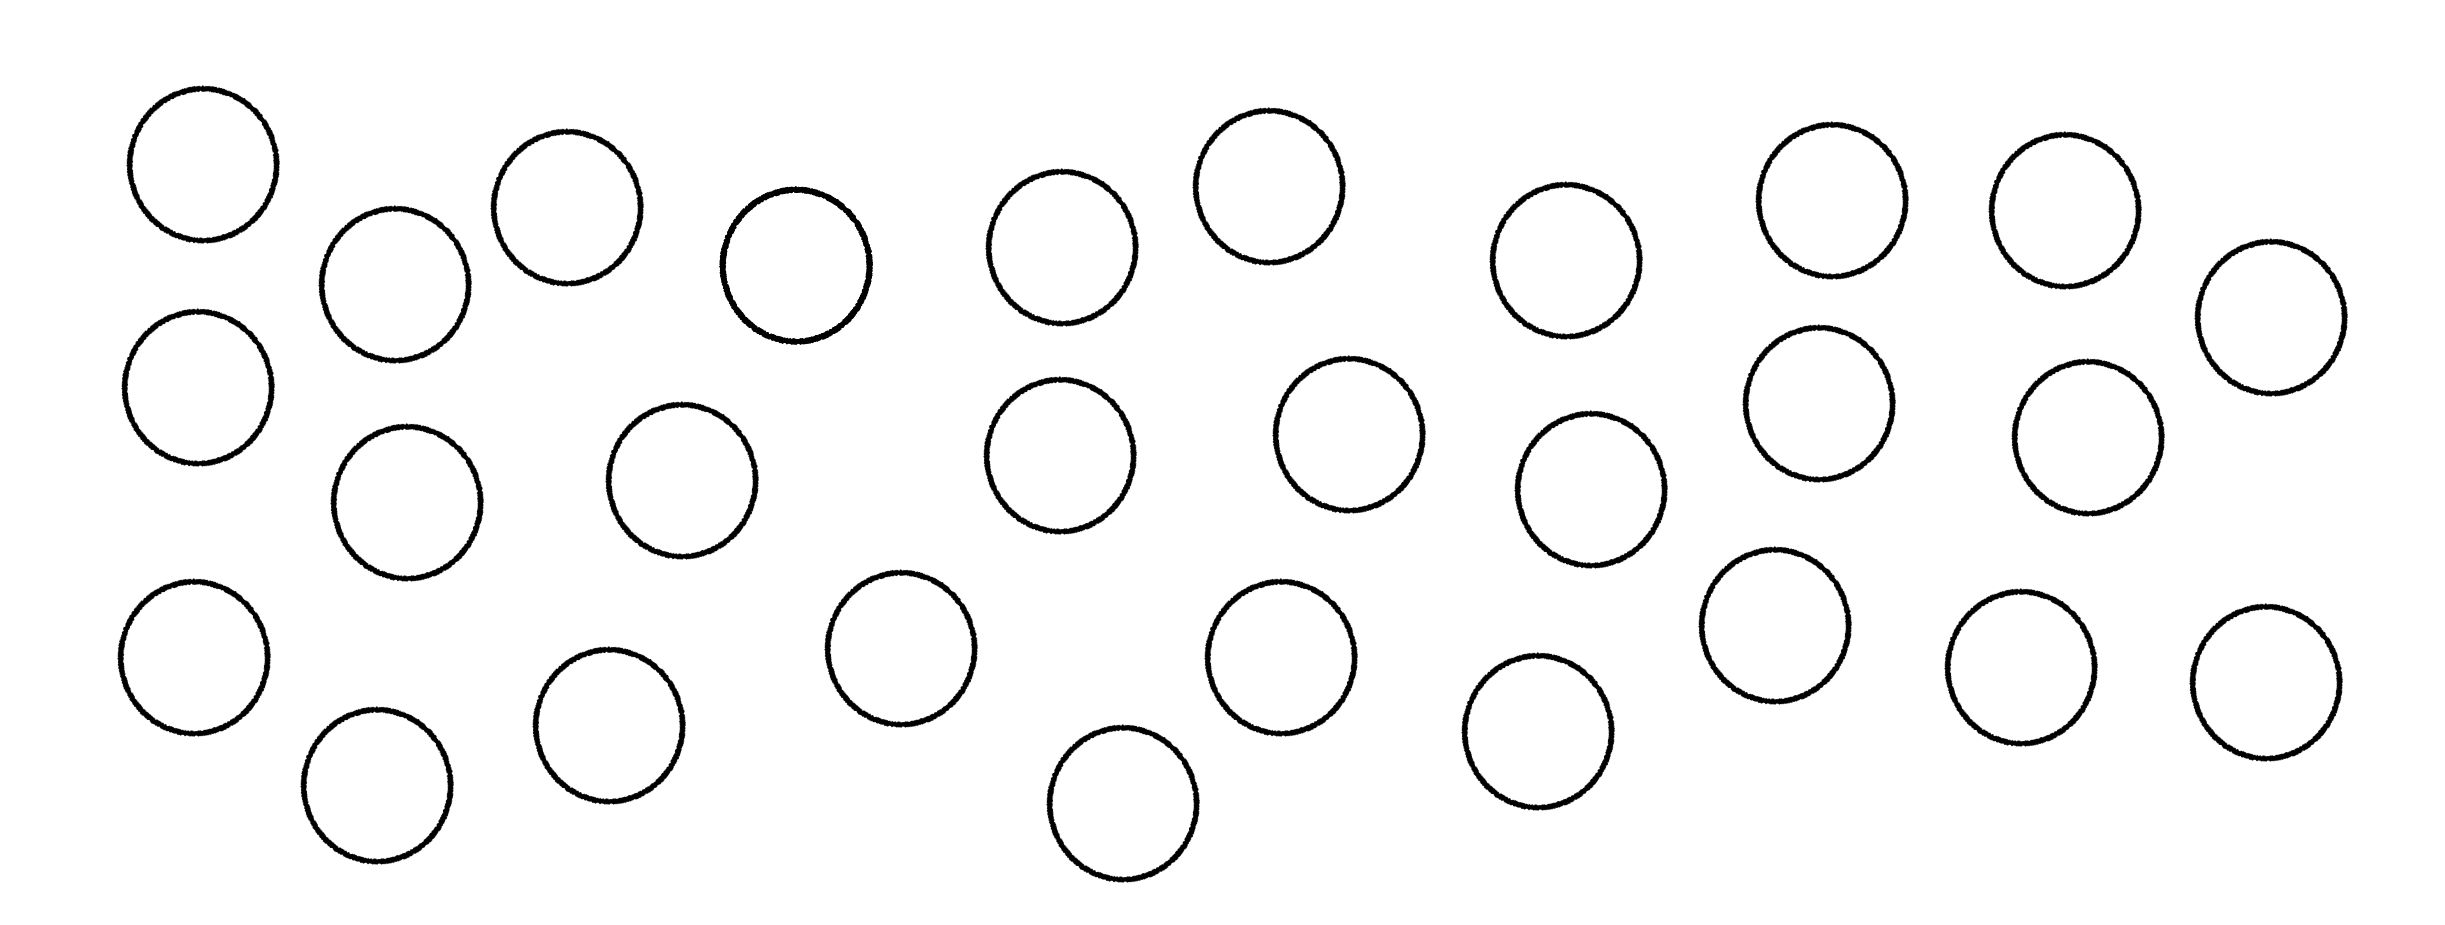
\includegraphics[width=\textheight ,
%    keepaspectratio]{surfacet1.jpg}}{test.mp4}

% \end{frame}
%%%%%%%%%%%%%%%%%%%%%%%%%%%%%%%%%%%%%%%%%%%%%%%%%%%%%%%%%%%%%%%%%%%

%%%%%%%%%%%%%%%%%%%%%%%%%%%%%%%%%%%%%%%%%%%%%%%%%%%%%%%%%%%%%%%%%%%


%%%%%%%%%%%%%%%%%%%%%%%%%%%%%%%%%%%%%%%%%%%%%%%%%%%%%%%%%%%%%%%
\section{Sound}

\begin{frame}
\frametitle{Sound}

Is an interpretation of our brain of a physical sensation that stimulate our ears, that is, a longitudinal wave.

\pause

\vspace{3mm}

We must consider...

\pause
\begin{itemize}
\item Source $\rightarrow$ vibrating object.

\pause
\item Needs mater to spread.

\pause
\item The energy is transferred as longitudinal waves.

\pause
\item Detection $\rightarrow$ ears, microphone, etc.
\end{itemize}


  \end{frame}


%%%%%%%%%%%%%%%%%%%%%%%%%%%%%%%%%%%%%%%%%%%%%%%%%%%%%%%%%%%%%%%
\subsection{Characteristics}

\begin{frame}
\frametitle{Sound Speed}

The velocity of the propagation of sound in a medium is,

\begin{equation}
v=\sqrt{\frac{B}{\rho}}
\end{equation}

\pause

where $B$ is the Bulk modulus, defined by

\begin{equation*}
\Delta P=-B\frac{\Delta V}{V}
\end{equation*}

\pause
change in pressure \pause $\rightarrow$ change of volume 

 



  \end{frame}



%%%%%%%%%%%%%%%%%%%%%%%%%%%%%%%%%%%%%%%%%%%%%%%%%%%%%%%%%%%%%%%

\begin{frame}
\frametitle{Sound Speed}


  \begin{center}
  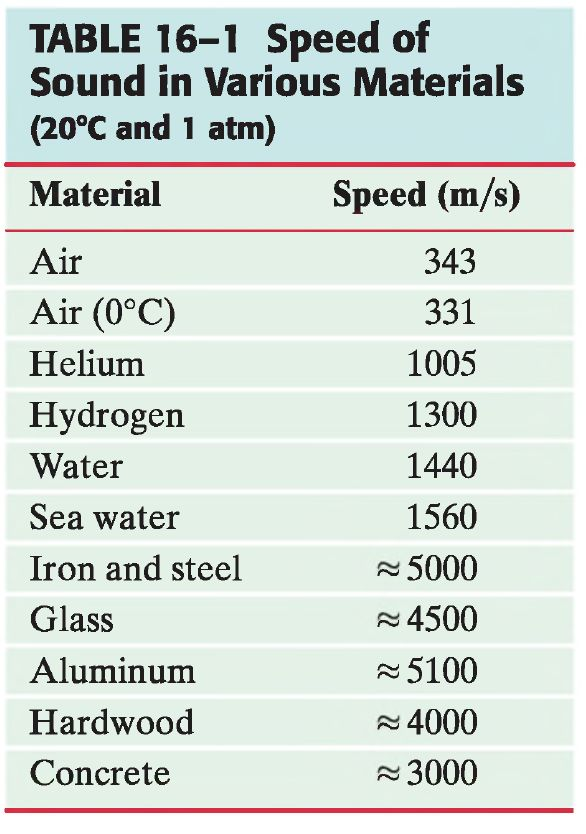
\includegraphics[height=2.4in]{images4/sound_speed.jpg}
\end{center}




  \end{frame}



%%%%%%%%%%%%%%%%%%%%%%%%%%%%%%%%%%%%%%%%%%%%%%%%%%%%%%%%%%%%%%%
\subsection{Mathematical Description}


\begin{frame}
\frametitle{Pressure Waves}

A sound wave is a longitudinal wave described by,

\pause

\begin{equation*}
D(x,t)=Asin(kx-\omega t) \pause ~~\textcolor{mypink1}{displacement}
\end{equation*}

\pause
  \begin{center}
  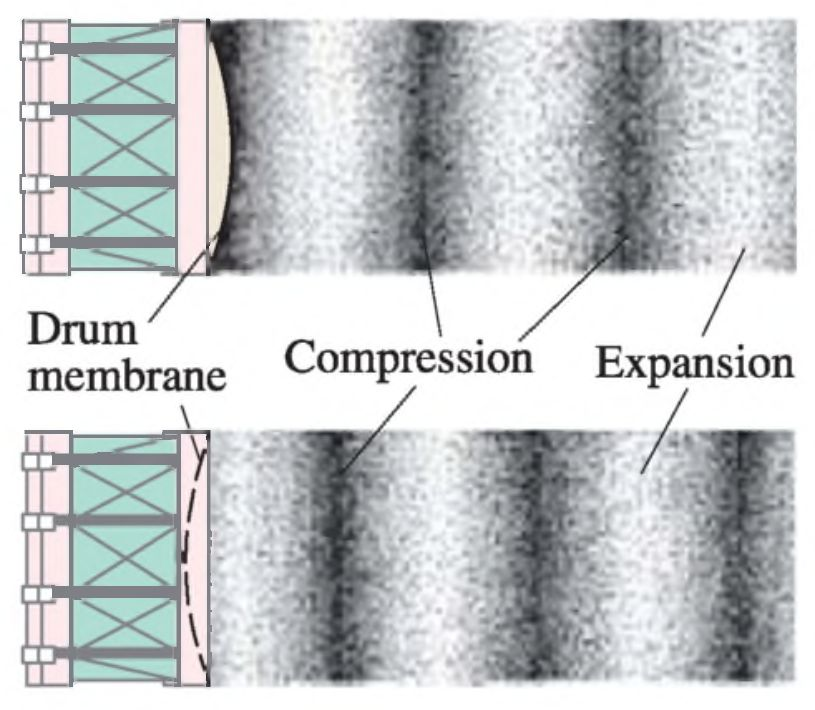
\includegraphics[height=1.4in]{images4/5.jpg}
\end{center}

\pause
The variation of pressure is easier to measure.
  \end{frame}

%%%%%%%%%%%%%%%%%%%%%%%%%%%%%%%%%%%%%%%%%%%%%%%%%%%%%%%%%%%%%%%

\begin{frame}
\frametitle{Pressure Waves}

The displacement and pressure are $\frac{\pi}{2}$ out of phase.
  \begin{center}
  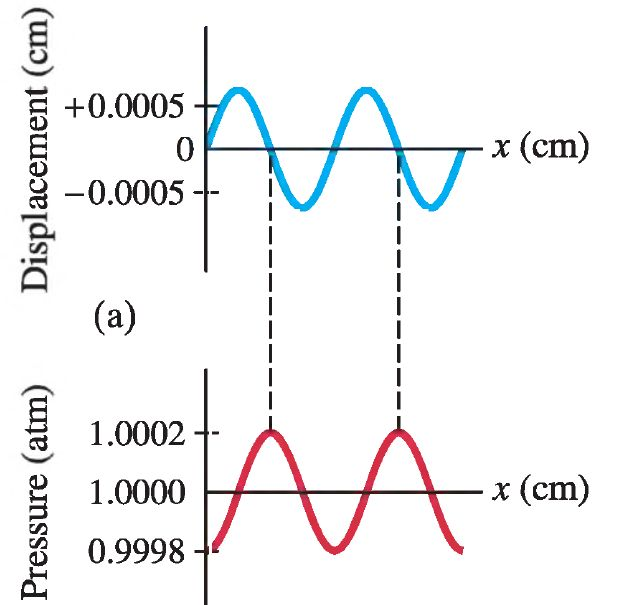
\includegraphics[height=2.in]{images4/soundwave.jpg}
\end{center}

  \end{frame}



%%%%%%%%%%%%%%%%%%%%%%%%%%%%%%%%%%%%%%%%%%%%%%%%%%%%%%%%%%%%%%%

\begin{frame}
\frametitle{Pressure Waves}
If we know $D(x,t)$ \pause what is the pressure wave?  \pause \textcolor{mypink1}{use the Bulk modulus}

\pause





   \begin{columns}[c]
   \column{1.8in}  % slides are 3in high by 5in wide
  
  \begin{center}
  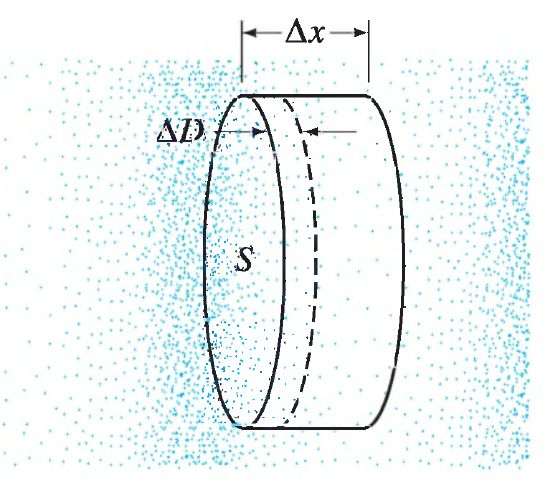
\includegraphics[height=1.5in]{images4/Pressurewave.jpg}
\end{center}

   \column{2.2in}

   \begin{equation*}
    \Delta P=-B\frac{\Delta V}{V}
    \end{equation*}
    
    \pause
    \begin{equation*}
      V=S\Delta x
      \end{equation*}
    

\pause


\begin{equation*}
  \Delta V=S\Delta D
\end{equation*}


\pause


\begin{equation*}
\rightarrow \Delta P=-B\frac{S\Delta D}{S\Delta x}
\end{equation*}


   \end{columns}




  \end{frame}
%%%%%%%%%%%%%%%%%%%%%%%%%%%%%%%%%%%%%%%%%%%%%%%%%%%%%%%%%%%%%%%

\begin{frame}
\frametitle{Pressure Waves}
Taking the limit for $\Delta x\rightarrow 0$

\begin{equation*}
\Delta P=-B\frac{\partial  D}{\partial x}
\end{equation*}



\begin{equation*}
  \rightarrow \frac{\partial  D}{\partial x}=kA cos(kx-\omega t)
\end{equation*}



\begin{equation}
  \rightarrow \boxed{\textcolor{mypink1}{\Delta P=-BkA cos(kx-\omega t)}}
\end{equation}

The pressure amplitude is:


\begin{equation}
\Delta P_M=BkA 
\end{equation}

  \end{frame}



%%%%%%%%%%%%%%%%%%%%%%%%%%%%%%%%%%%%%%%%%%%%%%%%%%%%%%%%%%%%%%%

\begin{frame}
\frametitle{Pressure Waves}
Using the relations,


\begin{equation*}
v=\sqrt{\frac{B}{\rho}}, \ k=\frac{2\pi f}{v}
\end{equation*}

\begin{equation}
\Delta P_M=BkA =\boxed{2\pi v \rho f A}
\end{equation}

  \end{frame}

  %%%%%%%%%%%%%%%%%%%%%%%%%%%%%%%%%%%%%%%%%%%%%%%%%%%%%%%%%%%%%%%

\begin{frame}
  \frametitle{Sound Characteristics}
  
  To describe the sound, we have to consider two aspects,
  \vspace{5mm}
  
  \pause
  
  \begin{itemize}
  \item Loudness$\rightarrow$ Intensity ($\frac{E}{tS}$)
  \pause
  
  \item Pitch $\rightarrow$   frequency
  \end{itemize}
  
  \pause
  
  \vspace{3mm}
  
  The audible range by humans  is $20$~Hz to $20000$~Hz
  
    \end{frame}
%%%%%%%%%%%%%%%%%%%%%%%%%%%%%%%%%%%%%%%%%%%%%%%%%%%%%%%%%%%%%%%

\begin{frame}
\frametitle{Intensity of sound}


We are going  to define a new measurement unit that relates the intensity with loudness.
\vspace{3mm}
\pause

\begin{equation*}
I=\frac{Energy}{time~Surface}, \ \ [I]=\frac{W}{m^2}
\end{equation*}


\begin{itemize}
\item Intensity $\rightarrow$ Physically meassurable quantity.
\pause

\item Loudness $\rightarrow$ Subjective sensation. 
\end{itemize}
\pause
\vspace{3mm}

In terms of intensity, the Human ear can hear  
\vspace{3mm}
\pause

form $10^{-12}~\frac{W}{m^2}$ to $1~\frac{W}{m^2}$.

\vspace{3mm}
\pause
Then, we are going to define this new unit  in log scale.

  \end{frame}







%%%%%%%%%%%%%%%%%%%%%%%%%%%%%%%%%%%%%%%%%%%%%%%%%%%%%%%%%%%%%%%

\begin{frame}
\frametitle{Decibel}

We are going to define one decibel ($1~dB$) as,
\pause

\begin{equation}
\beta~ (in ~dB)=10 log\frac{I}{I_0}
\end{equation}

\pause

where $log$ is in base $10$, and $I_0$ is the intensity of a chosen reference level.
\pause

\begin{equation}
I_0=10^{-12}~\frac{W}{m^2}, \ minimum~audible~intensity
\end{equation}

  \end{frame}



%%%%%%%%%%%%%%%%%%%%%%%%%%%%%%%%%%%%%%%%%%%%%%%%%%%%%%%%%%%%%%%

\begin{frame}
\frametitle{Decibel}

Example: 

\vspace{3mm}

What is  the level of a sound whose intensity is $I=10^{-10}$~$\frac{W}{m^2}$?

\pause

\begin{equation}
\beta =10 log\left(\frac{10^{-10}}{10^{-12}}\right)=10log100=20~dB
\end{equation}

\pause
\vspace{3mm}
At the threshold of hearing?  $I=10^{-12}$~$\frac{W}{m^2}$?

\begin{equation}
\beta =10 log\left(\frac{10^{-12}}{10^{-12}}\right)=10log1=0
\end{equation}

  \end{frame}

%%%%%%%%%%%%%%%%%%%%%%%%%%%%%%%%%%%%%%%%%%%%%%%%%%%%%%%%%%%%%%%

\begin{frame}
\frametitle{Decibel}

An increase in $I$ by a factor $10$ is equivalent to an increase in $10$~dB.
\pause

\begin{equation*}
I'=10I\rightarrow \beta'=10 log \frac{10I}{I_0}=10[log 10+log\frac{I}{I_0} ]
\end{equation*}
\pause
\begin{equation*}
\rightarrow\beta'=10~dB+10log\frac{I}{I_0} 
\end{equation*}
\pause

An increase in $I$ by a factor $10^2$ is equivalent to an increase in $20$~dB and so on...



  \end{frame}

%%%%%%%%%%%%%%%%%%%%%%%%%%%%%%%%%%%%%%%%%%%%%%%%%%%%%%%%%%%%%%%

\begin{frame}
\frametitle{Decibel}

  \begin{center}
  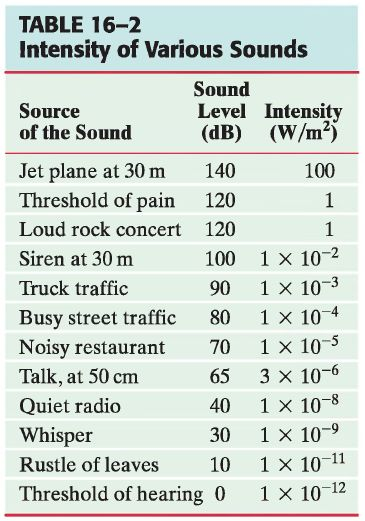
\includegraphics[height=2.5in]{images4/decibels.jpg}
\end{center}




  \end{frame}





%%%%%%%%%%%%%%%%%%%%%%%%%%%%%%%%%%%%%%%%%%%%%%%%%%%%%%%%%%%%%%%

\begin{frame}
\frametitle{Decibel}
Conceptual example:

\vspace{3mm}

A trumpeter plays at a sound level of $75~dB$. Three equally loud trumpet players join in. What is the new
sound level?

\pause

\begin{equation*}
\beta =10 log\frac{4 I_1}{I_0}
\end{equation*}


  \end{frame}




%%%%%%%%%%%%%%%%%%%%%%%%%%%%%%%%%%%%%%%%%%%%%%%%%%%%%%%%%%%%%%%

\begin{frame}
\frametitle{Decibel}
Conceptual example:

\vspace{3mm}

A trumpeter plays at a sound level of $75~dB$. Three equally loud trumpet players join in. What is the new
sound level?

\begin{equation*}
\beta =10 log\frac{4 I_1}{I_0}=10log(4)+10~log\frac{ I_1}{I_0}
\end{equation*}


  \end{frame}



%%%%%%%%%%%%%%%%%%%%%%%%%%%%%%%%%%%%%%%%%%%%%%%%%%%%%%%%%%%%%%%

\begin{frame}
\frametitle{Decibel}
Conceptual example:

\vspace{3mm}

A trumpeter plays at a sound level of $75~dB$. Three equally loud trumpet players join in. What is the new
sound level?

\begin{equation*}
\beta =10 log\frac{4 I_1}{I_0}=10log(4)+10~log\frac{ I_1}{I_0}=6.0~dB+75~dB=81~dB
\end{equation*}


  \end{frame}


  %%%%%%%%%%%%%%%%%%%%%%%%%%%%%%%%%%%%%%%%%%%%%%%%%%%%%%%%%%%%%%%



\begin{frame}
  \frametitle{Equally Tempered Chromatic Scale}
  
  PITCH $\leftrightarrow$ FREQUENCY
  
  
    \begin{center}
    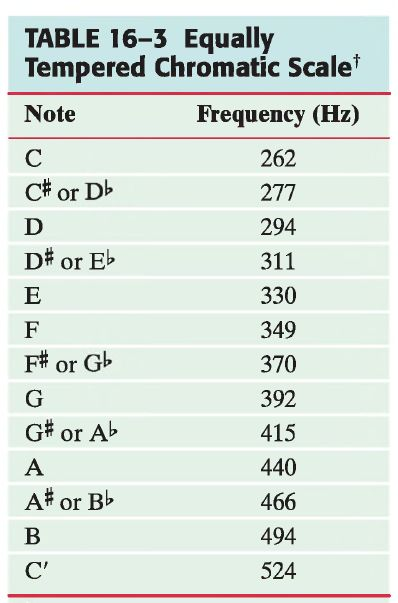
\includegraphics[height=2.1in]{images4/scale.jpg}
  \end{center}
  
  
  
    \end{frame}

    

%%%%%%%%%%%%%%%%%%%%%%%%%%%%%%%%%%%%%%%%%%%%%%%%%%%%%%%%%%%%%%%
\subsection{Sources of Sound}

\begin{frame}
\frametitle{Sources of Sound}

\begin{itemize}
  \item VIBRATING OBJECTS \pause
  \item PUSHES THE MEDIUM \pause PRODUCES SOUND WAVES \pause
  \item FEQUENCIE = SOURCE FREQUENCY \pause
  \item SPEED DEPENDS ON THE MEDIUM \pause
\end{itemize}








  \end{frame}






%%%%%%%%%%%%%%%%%%%%%%%%%%%%%%%%%%%%%%%%%%%%%%%%%%%%%%%%%%%%%%%



\begin{frame}
\frametitle{Stringed Instruments}

\begin{itemize}
  \item Standing waves are the basis for all stringed instruments. \pause
  \item  Pitch= fundamental frequency $f=v/2\ell$ \pause
  \item Harmonics= $f_n=nf_1=n\frac{v}{2\ell}$ \pause
\end{itemize}





  \end{frame}


%%%%%%%%%%%%%%%%%%%%%%%%%%%%%%%%%%%%%%%%%%%%%%%%%%%%%%%%%%%%%%%



\begin{frame}
\frametitle{Stringed Instruments}
  \textcolor{mypink1}{$v,f$ fixed. \pause $\ell$ variable}

  

  \begin{figure}[h!]
    \begin{center}
      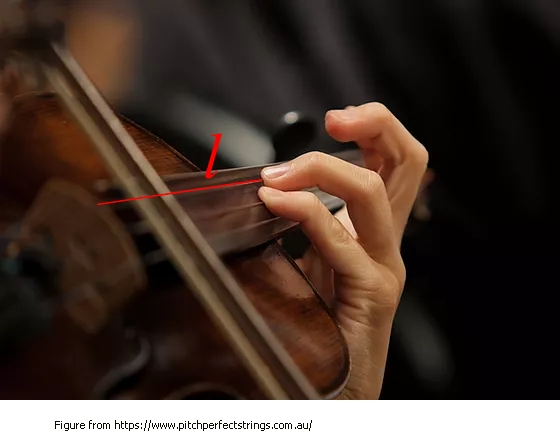
\includegraphics[height=2.in]{images4/pitch.jpg}
    \end{center}
  \end{figure}



\end{frame}
%%%%%%%%%%%%%%%%%%%%%%%%%%%%%%%%%%%%%%%%%%%%%%%%%%%%%%%%%%%%%%%


\begin{frame}
\frametitle{Stringed Instruments}


 Different $\mu\rightarrow$ different pitch

\pause


\begin{equation}
v=\sqrt{\frac{F_T}{\mu}}
\end{equation}

\vspace{3mm}
\pause

 heavier string \pause  lower $v$ and  frequency. 


\vspace{3mm}
\pause

The tension $F_T$ may also be different.  Adjusting the tension $\rightarrow$ tuning the pitch of each string.


  \end{frame}






%%%%%%%%%%%%%%%%%%%%%%%%%%%%%%%%%%%%%%%%%%%%%%%%%%%%%%%%%%%%%%%



% \begin{frame}
% \frametitle{Piano Strings}

% Example:

% \vspace{3mm}

% The highest key on a piano corresponds to a frequency about $150$ times that of the lowest key. If the string for the highest note
% is $5.0~cm$ long, how long would the string for the lowest note have to be if it had the same mass per unit length and was under the same tension?

% \pause

% \begin{equation}
% f_n=n\frac{v}{2\ell}
% \end{equation}
% \pause


% \begin{equation}
% \rightarrow \frac{\ell_L}{\ell_H}=\frac{f_H}{f_L}=150\rightarrow\ell_L=\frac{f_H}{f_L}=150\ell_H=750~cm
% \end{equation}


%   \end{frame}



% %%%%%%%%%%%%%%%%%%%%%%%%%%%%%%%%%%%%%%%%%%%%%%%%%%%%%%%%%%%%%%%



% \begin{frame}
% \frametitle{Piano Strings}


% The longer strings of lower frequency are made heavier, of higher mass
% per unit length, so even on grand pianos the strings are less than 3 m long.

%   \end{frame}


%%%%%%%%%%%%%%%%%%%%%%%%%%%%%%%%%%%%%%%%%%%%%%%%%%%%%%%%%%%%%%%



% \begin{frame}
% \frametitle{Example}

% Frequencies and wavelengths in the violin:
% \vspace{3mm}


% A $0.32~m$ long violin string is tuned to play A above middle C at 440 Hz. (a) What is the
% wavelength of the fundamental string vibration, and (b) what are the frequency
% and wavelength of the sound wave produced? (c) Why is there a difference?

%   \end{frame}


%%%%%%%%%%%%%%%%%%%%%%%%%%%%%%%%%%%%%%%%%%%%%%%%%%%%%%%%%%%%%%%



\begin{frame}
\frametitle{Sound Amplification}


\begin{enumerate}
  \item Strings are set into vibration \pause
  \item  the sounding board or box is set  into vibration as well \pause
  \item  much greater area in contact with the air \pause
  \item  has much greater area in contact with the air, it can
  produce a  \pause
\end{enumerate}




  \end{frame}


%%%%%%%%%%%%%%%%%%%%%%%%%%%%%%%%%%%%%%%%%%%%%%%%%%%%%%%%%%%%%%%



% \begin{frame}
% \frametitle{Wind Instruments}

% Instruments such as woodwinds, the brasses, and the pipe organ produce sound
% from the vibrations of standing waves in a column of air within a tube.
% \pause 
% \vspace{3mm}

% Standing waves can occur in the air of any cavity, but the frequencies present can be 
% complicated.
% \pause 
% \vspace{3mm}

% We are going to study a narrow tube of a flute or an organ pipe. 
% \pause 
% \vspace{3mm}

% Source $\rightarrow$ vibrating reed / vibrating lip /  stream against one edge leading to turbulence
% \pause 
% \vspace{3mm}

% The air within the tube vibrates with a variety of frequencies, but only frequencies that
% correspond to standing waves will persist.

%   \end{frame}


%%%%%%%%%%%%%%%%%%%%%%%%%%%%%%%%%%%%%%%%%%%%%%%%%%%%%%%%%%%%%%%



\begin{frame}
\frametitle{Modes of vibration for an open tube}

  \begin{center}
  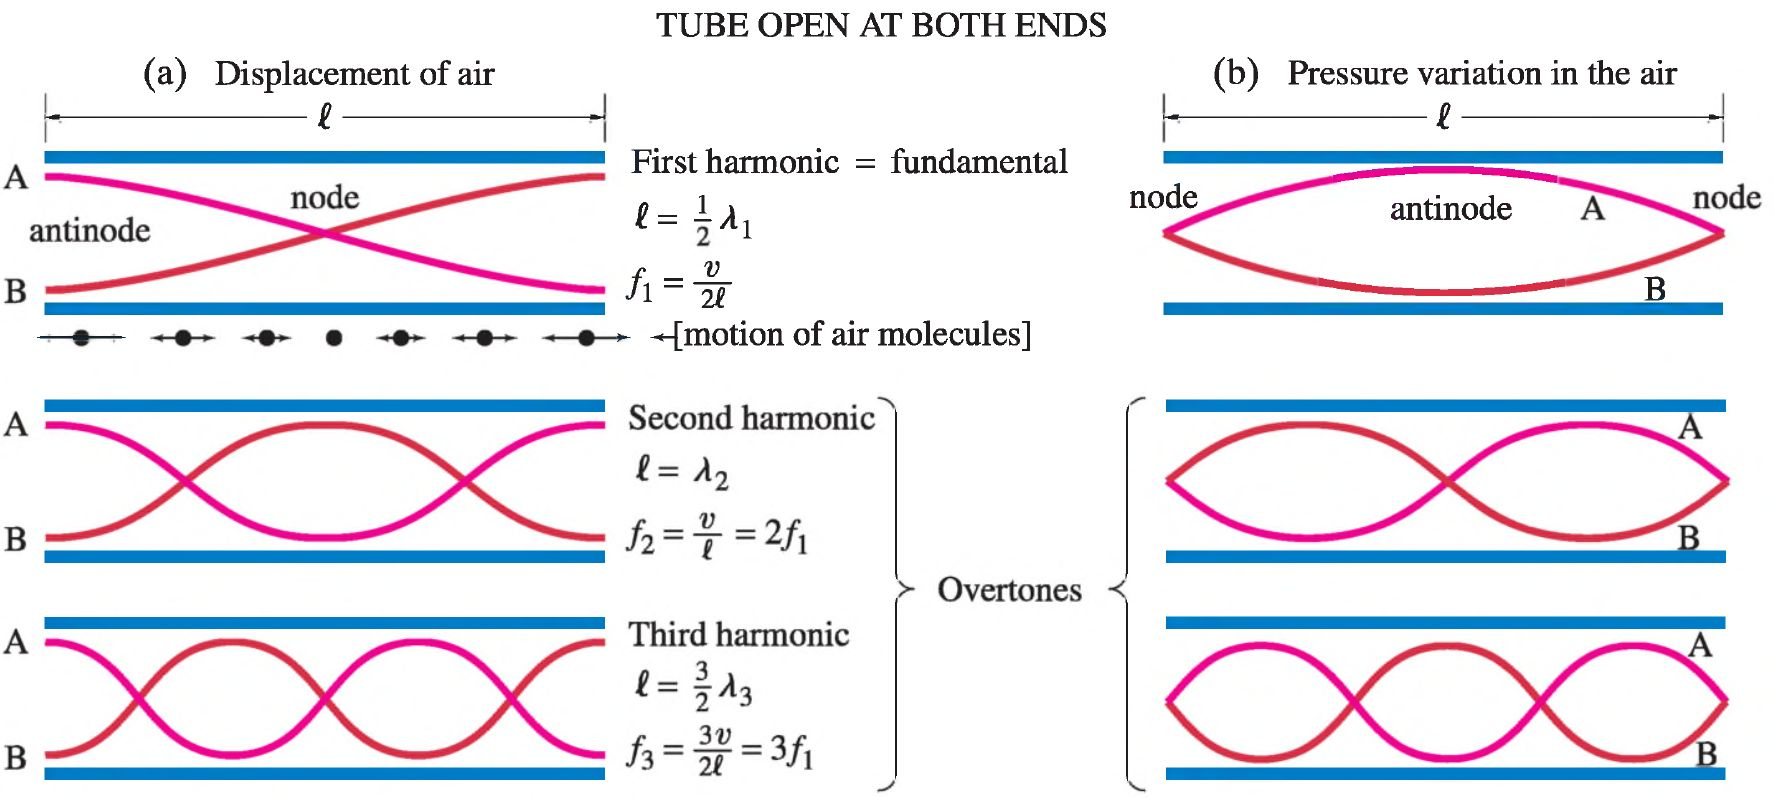
\includegraphics[height=2.in]{images4/tubeopen.jpg}
\end{center}


  \end{frame}




%%%%%%%%%%%%%%%%%%%%%%%%%%%%%%%%%%%%%%%%%%%%%%%%%%%%%%%%%%%%%%%



% \begin{frame}
% \frametitle{Modes of vibration for an open tube}

% In terms of he displacement $D(x,t)$:

% \begin{itemize}
% \item Antinodes at both ends.
% \pause
% \item  There must be at least one node within an open tube.
% if there is to be a standing wave at all.
% \pause
% \item Fundamental frequency $\rightarrow$ single node. 
% \pause
% \item Distance between two successive nodes (or antinodes),  is  $1/2\lambda\rightarrow \lambda=2\ell$.
% \pause
% \item Fundamental frequency: $f_0=v /\lambda=v/2\ell$, $v$ is the velocity of sound in the air.
% \pause
% \item  $f_n=n v /\lambda=n v/2\ell$.
% \end{itemize}


%   \end{frame}

% %%%%%%%%%%%%%%%%%%%%%%%%%%%%%%%%%%%%%%%%%%%%%%%%%%%%%%%%%%%%%%%

 \begin{frame}
 \frametitle{Modes of vibration for a tube closed at one end}

   \begin{center}
   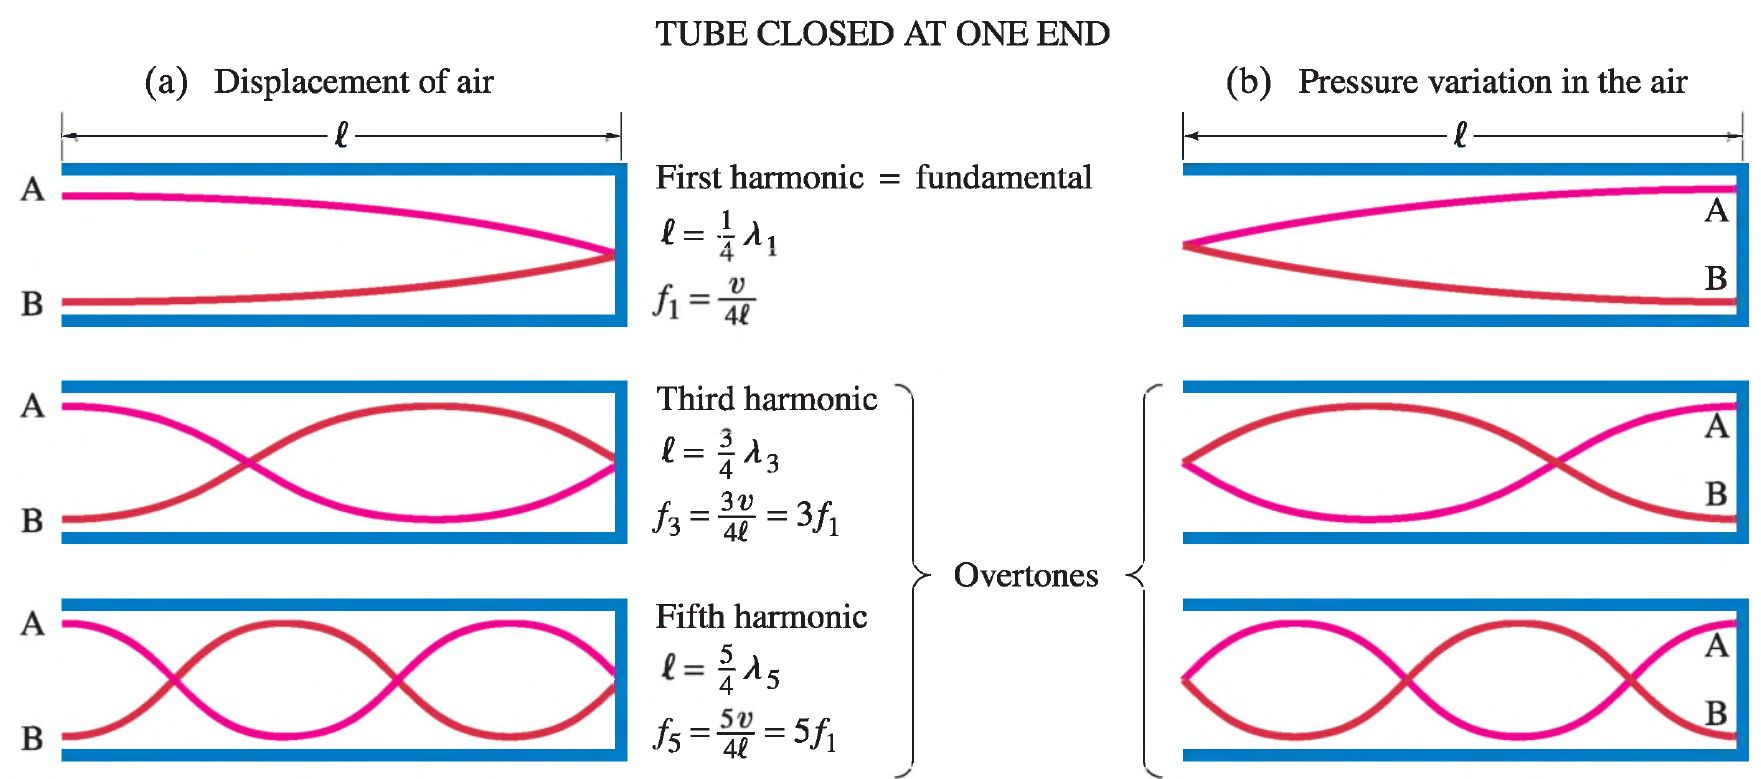
\includegraphics[height=2.in]{images4/tubeclose.jpg}
 \end{center}


   \end{frame}


% %%%%%%%%%%%%%%%%%%%%%%%%%%%%%%%%%%%%%%%%%%%%%%%%%%%%%%%%%%%%%%%

% \begin{frame}
% \frametitle{Modes of vibration for a tube closed at one end}

% In terms of $D(x,t)$:
% \vspace{3mm}

% \begin{itemize}
% \item There is always a displacement node at the closed end.
% \pause
 
% \item Distance between a node and the nearest antinode $\lambda/4$
% \pause

% \item Only the odd harmonics are present in a closed tube: the overtones have frequencies equal to $3f_1$,$5f_1$, $7f_1$,...
% \pause

% \item  There is no way for waves with $2f_1$, $4f_1$, $6f_1$


% \end{itemize}



%   \end{frame}




%%%%%%%%%%%%%%%%%%%%%%%%%%%%%%%%%%%%%%%%%%%%%%%%%%%%%%%%%%%%%%%



% \begin{frame}
% \frametitle{Modes of vibration for a tube closed at one end}

% In terms of the pressure in the air:
% \vspace{3mm}

% \begin{itemize}

% \item Air in a wave compressed $\rightarrow$ higher pressure.
% \pause

% \item Wave expansion (or rarefaction) $\rightarrow$ lower pressure.
% \pause

% \item The open end of a tube is open to the atmosphere $\rightarrow$ the pressure  remains at the outside atmospheric pressure (node).
% \pause

% \item  If a tube has a closed end  $\rightarrow$  the pressure  alternates to be above or below atmospheric pressure (antinode). 
% \end{itemize}





%   \end{frame}








%%%%%%%%%%%%%%%%%%%%%%%%%%%%%%%%%%%%%%%%%%%%%%%%%%%%%%%%%%%%%%%



% \begin{frame}
% \frametitle{Modes of vibration for a tube closed at one end}

% Example:
% \vspace{3mm}

% Organ pipes. What will be the fundamental frequency and first
% three overtones for a $26~cm$ long organ pipe at $20°C$  if it is (a) open and (b) closed?

%   \end{frame}

%%%%%%%%%%%%%%%%%%%%%%%%%%%%%%%%%%%%%%%%%%%%%%%%%%%%%%%%%%%%%%%

% \begin{frame}

% \frametitle{Modes of vibration for a tube closed at one end}

% Example:
% \vspace{3mm}

% A flute is designed to play middle C (262 Hz) as the
% fundamental frequency when all the holes are covered. Approximately how long
% should the distance be from the mouthpiece to the far end of the flute? (This is
% only approximate since the antinode does not occur precisely at the mouthpiece.)
% Assume the temperature is 20°C.

%   \end{frame}
%%%%%%%%%%%%%%%%%%%%%%%%%%%%%%%%%%%%%%%%%%%%%%%%%%%%%%%%%%%%%%%

% \begin{frame}
% \frametitle{modes of vibration for an open tube}

% Example:
% \vspace{3mm}


% To see why players of wind instruments “warm up” their instruments (so they
% will be in tune), determine the fundamental frequency of the flute  when
% all holes are covered and the temperature is 10°C instead of 20°C.


%   \end{frame}


%%%%%%%%%%%%%%%%%%%%%%%%%%%%%%%%%%%%%%%%%%%%%%%%%%%%%%%%%%%%%%%


\subsection{Quality of Sound, and Noise;
Superposition}

\begin{frame}
\frametitle{Quality of sound}

SOUND \pause $\rightarrow$ LOUDNESS \pause PITCH and \textcolor{mypink1}{QUALITY}

\pause
\vspace{3mm}

QUALITY \pause $\leftrightarrow$ Harmonics (combination of sins) 

\pause
\vspace{3mm}

$\rightarrow $ SHAPES OF THE WAVES

\end{frame}



%%%%%%%%%%%%%%%%%%%%%%%%%%%%%%%%%%%%%%%%%%%%%%%%%%%%%%%%%%%%%%%




\begin{frame}
\frametitle{Quality of sound}

WAVE:

\begin{equation*}
  f(t)=\sum^{N}_{n=1} A_n cos\left(\frac{2n\pi t}{L}\right)
\end{equation*}

\pause
\vspace{5mm}

\begin{equation*}
  A_n(w_n)~~Determines~~wave~~shape
\end{equation*}

\end{frame}



%%%%%%%%%%%%%%%%%%%%%%%%%%%%%%%%%%%%%%%%%%%%%%%%%%%%%%%%%%%%%%%


\begin{frame}
\frametitle{Sound spectra for different instruments}
\begin{center}
  $A_n$ vs. $w_n$
\end{center}


\begin{columns}[c]
  \column{2in}  % slides are 3in high by 5in wide

  \begin{figure}[h!]
    \begin{center}
      \includegraphics[height=1.8in]{images4/violin.png}
    \end{center}
  \end{figure}
  
  \column{2in}

  \begin{figure}[h!]
    \begin{center}
      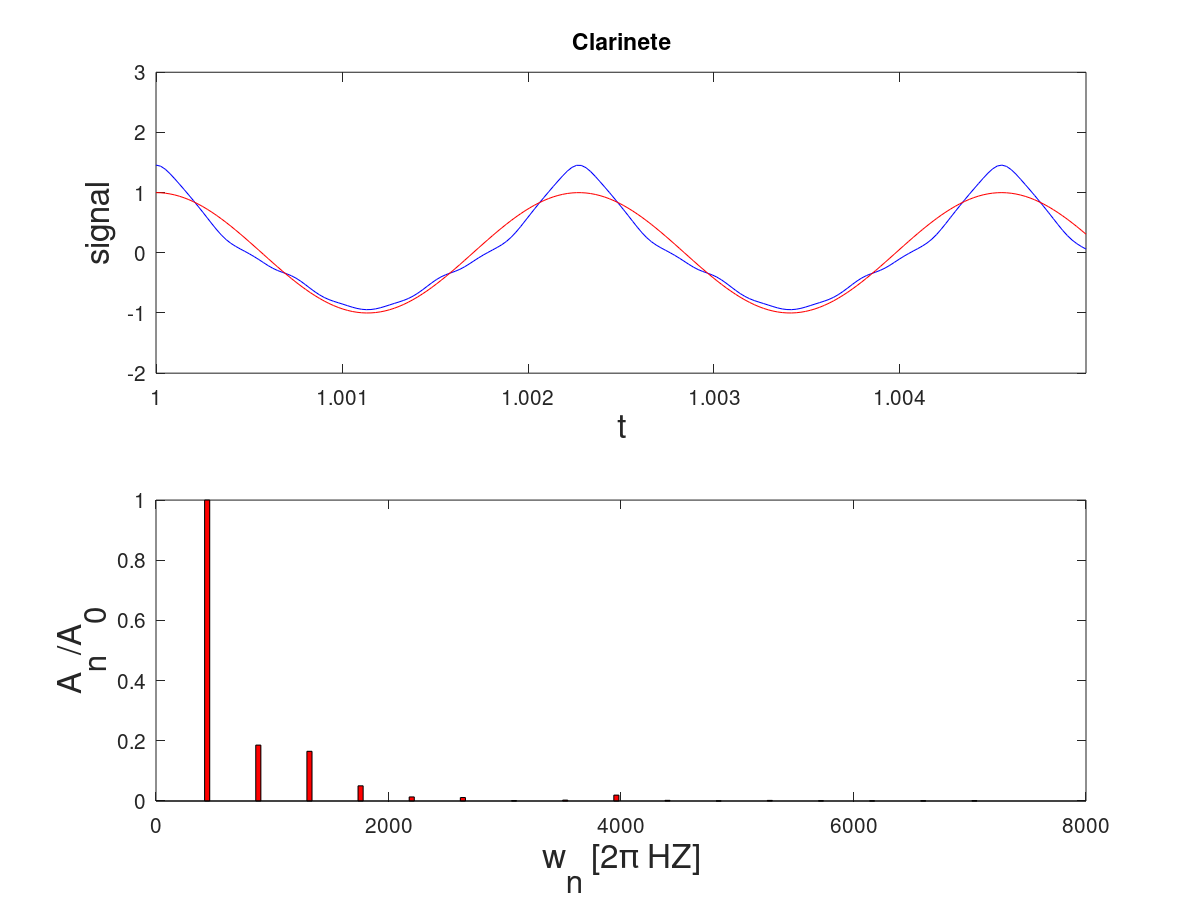
\includegraphics[height=1.8in]{images4/Clarinete.png}
    \end{center}
  \end{figure}
  

  \end{columns}


  \end{frame}


%%%%%%%%%%%%%%%%%%%%%%%%%%%%%%%%%%%%%%%%%%%%%%%%%%%%%%%%%%%%%%%

\begin{frame}
  \frametitle{Beats—Interference in Time}
  
  TWO SOURCES CLOSE IN FREQUENCY 
  \pause
  \vspace{5mm}

    \begin{center}
    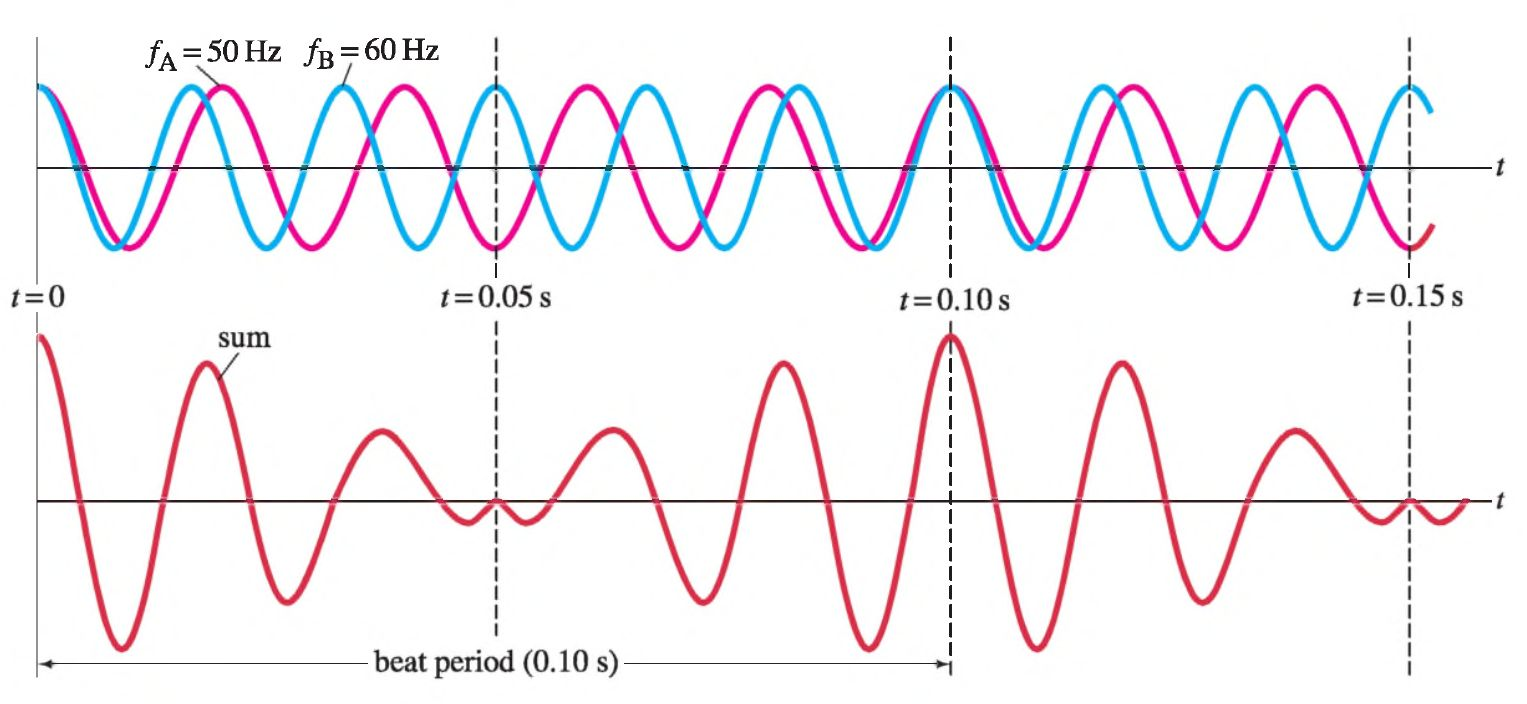
\includegraphics[height=1.7in]{images4/beats.jpg}
  \end{center}
  
  
  
    \end{frame}
  
  

  
  %%%%%%%%%%%%%%%%%%%%%%%%%%%%%%%%%%%%%%%%%%%%%%%%%%%%%%%%%%%%%%%
  
  \begin{frame}
  \frametitle{Beats, Interference in Time}
  
  
  At a fixed point in space:
  
  \begin{equation*}
  D_1=Asin(2\pi f_1t)
  \end{equation*}
  
  \pause
  \begin{equation*}
  D_2=Asin(2\pi f_1t)
  \end{equation*}
  \pause
  
  The resultant displacement is,
  
  \pause
  
  \begin{equation*}
  D=D_1+D_2=A[Asin(2\pi f_1t)+sin(2\pi f_1t)]
  \end{equation*}

  
    \end{frame}
  
  
  %%%%%%%%%%%%%%%%%%%%%%%%%%%%%%%%%%%%%%%%%%%%%%%%%%%%%%%%%%%%%%%
  
  \begin{frame}
  \frametitle{Beats, Interference in Time}
  
  
  
  
  Using, $sin\theta_1+sin\theta_2=2sin\frac{1}{2}(\theta_1+\theta_2)cos\frac{1}{2}(\theta_1-\theta_2)$
  
  \pause
  
  \begin{equation}
  D=\left[2Acos2\pi\left(\frac{f_1-f_2}{2}\right)t\right] sin2\pi\left(\frac{f_1+f_2}{2}\right)t
  \end{equation}
  
    \end{frame}
  
  
  
  %%%%%%%%%%%%%%%%%%%%%%%%%%%%%%%%%%%%%%%%%%%%%%%%%%%%%%%%%%%%%%%
  
  \begin{frame}
  \frametitle{Beats, Interference in Time}
  
  
   The superposition frequency: $(f_1+ f_ 2)/2$.
  
  \pause
  \vspace{3mm}
  

   \begin{equation}
    Amplitude:  ~~ \left[2Acos2\pi\left(\frac{f_1-f_2}{2}\right)t\right] 
    \end{equation}

  

  \pause
  \vspace{3mm}
  
  $ \rightarrow$ two beats occur per cycle \pause $\rightarrow$ beat frequency is $f_1-f_2$.
  
  
    \end{frame}
  
  

    



%%%%%%%%%%%%%%%%%%%%%%%%%%%%%%%%%%%%%%%%%%%%%%%%%%%%%%%%%%%%%%%
 \end{document}
%%%%%%%%%%%%%%%%%%%%%%%%%%%%%%%%%%%%%%%%%%%%%%%%%%%%%%%%%%%%%%%